\section{方法}
\label{sec:method}

\subsection{基础模型与总体结构}

本文以Qwen3-VL-4B-Instruct\cite{Bai2025Qwen3VLTR}为基础模型，记为$F_{\Phi}$，其中$\Phi$包含视觉编码器、视觉Merger、词嵌入层和自回归语言模型的参数。模型接收图像$I$和问题文本$X$，生成答案$Y$。领域训练集记为$\mathcal{D}=\{(I_i,X_i,Y_i)\}_{i=1}^{N}$。QDPT在基础模型中加入参数为$\Theta$的Prompt适配器，固定$\Phi$，通过答案Token上的自回归负对数似然优化$\Theta$：

\begin{equation}
\mathcal{L}(\Theta)
=-\sum_{i=1}^{N}\sum_{t=1}^{|Y_i|}
\log p_{\Phi,\Theta}
\left(y_{i,t}\mid I_i,X_i,Y_{i,<t}\right),
\qquad \Phi\ \text{保持冻结}.
\end{equation}

训练时，梯度通过冻结层传回适配器，使Prompt能够调整后续Token的表示。

图\ref{fig:qdpt-global}展示从图像和问题输入到答案生成的整体流程。

\begin{figure}[t]
    \centering
    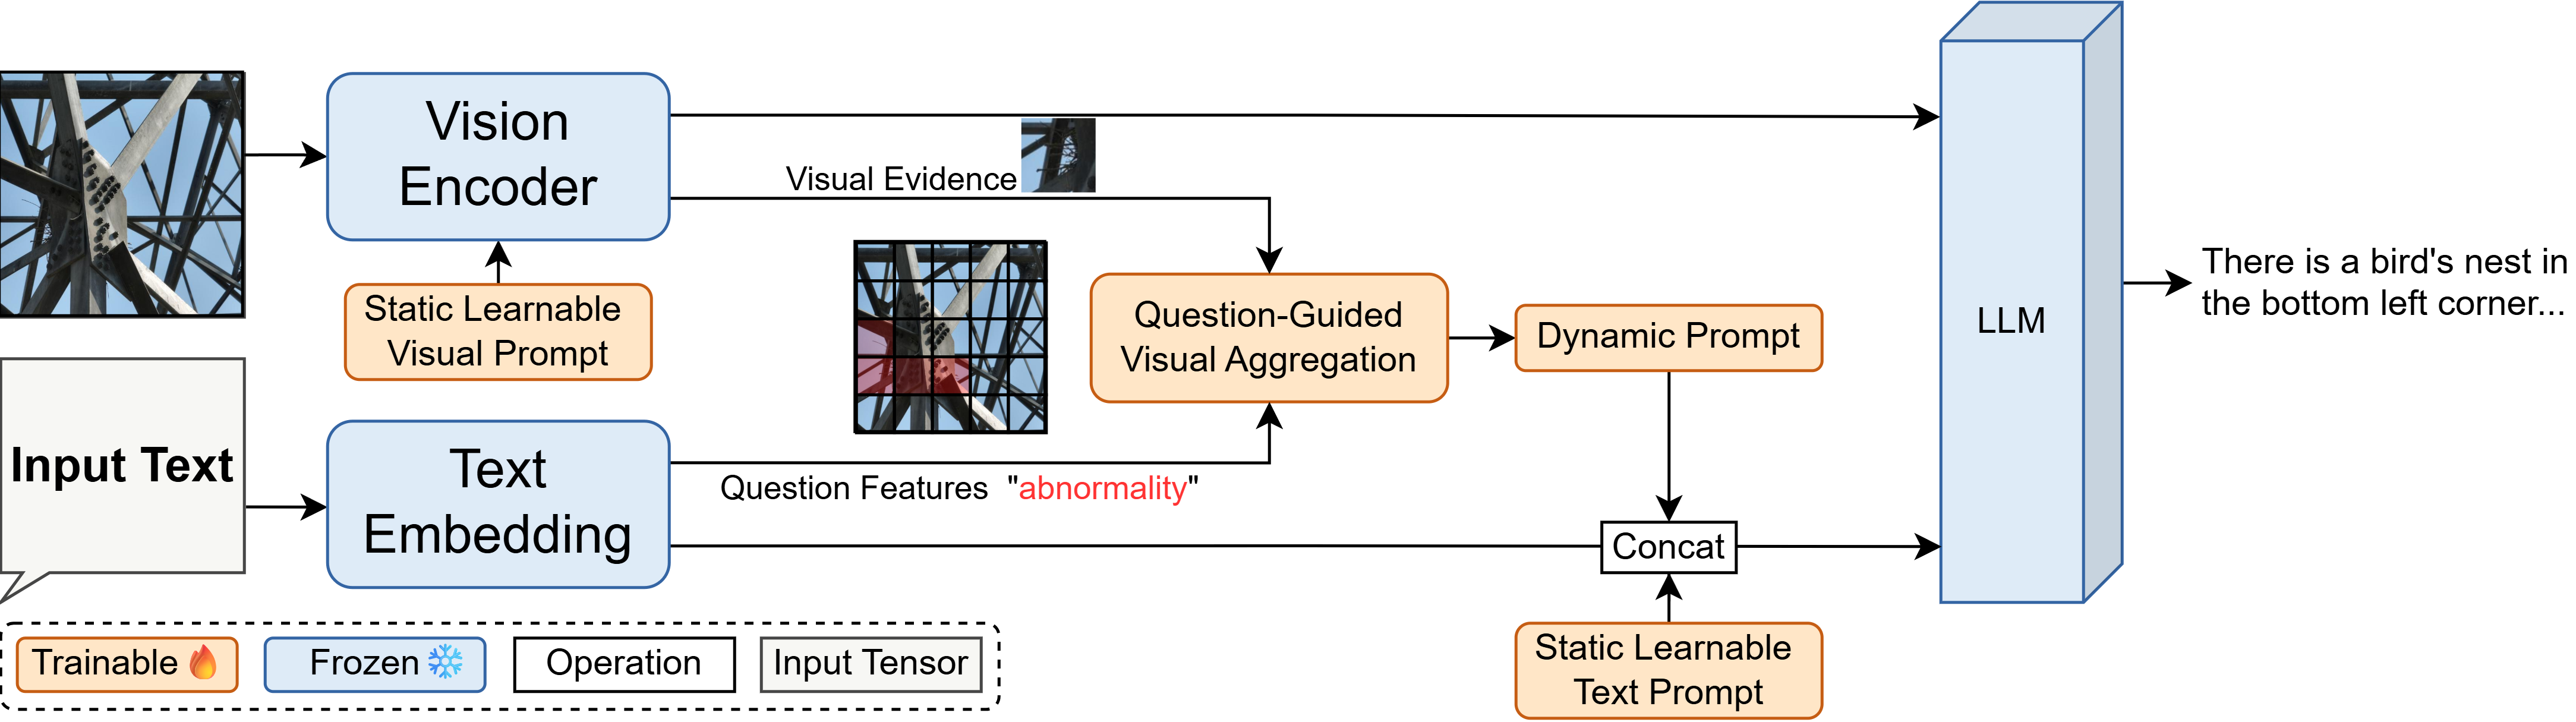
\includegraphics[width=\textwidth]{figures/qdpt_global_overview.png}
    \caption{QDPT整体框架。问题引导的视觉聚合生成样本相关的动态Prompt，静态Prompt在视觉侧与语言侧提供领域校准。蓝色模块的原有参数保持冻结，橙色模块为适配部分；视觉区域与问题关键词用于示意证据选择。}
    \label{fig:qdpt-global}
\end{figure}

视觉编码器包含24层Transformer，隐藏维度$d_v=1024$；语言模型包含36层Transformer，隐藏维度$d_l=2560$。基础模型总参数量约为4.445B。以下视觉层均采用从0开始的编号，索引17对应第18个Transformer Block。图像先经过冻结视觉编码器的第0至16层。模型在第17层加入静态视觉Prompt；该层计算结束后移除Prompt对应的输出，图像Token继续通过第18至23层和Merger。与此同时，QDPT对问题Token嵌入进行池化，生成10个Query，以进入第17层前的图像Token作为视觉K/V，计算Directional Workspace。映射层把所得表示转换为动态语言Prompt。送入LLM时，静态语言Prompt位于视觉Token之前，动态Prompt位于视觉Token与问题之间。

\begin{equation}
\begin{aligned}
P^{d}_{\Theta}(I,X)
&=A^{t}+g_{\theta}\!\left(\mathcal{W}_{\Theta}(H^{v}(I),H^{q}(X))\right),\\
p_{\Phi,\Theta}(Y\mid I,X)
&=\prod_{t=1}^{|Y|}p_{\Phi}\!\left(y_t\mid
[P^{t};M_{\Phi,P^{v}}(I);P^{d}_{\Theta}(I,X);T(X)],Y_{<t}\right).
\end{aligned}
\label{eq:qdpt-overall}
\end{equation}

其中$\mathcal{W}_{\Theta}$表示问题引导的视觉聚合，$g_{\theta}$将聚合表示映射到语言空间，$M_{\Phi,P^{v}}(I)$表示经静态视觉Prompt校准后的Merger输出，后文简记为$M(I)$。式\ref{eq:qdpt-overall}省略了聊天模板中的固定特殊Token。



\subsection{静态领域校准}

设第0至16个视觉Block输出的原始图像Token为
$H^{v}\in\mathbb{R}^{n_v\times d_v}$。QDPT采用视觉Prompt Tuning的连续Token形式\cite{jia2022visual}，维护18个可训练视觉Prompt
$P^{v}\in\mathbb{R}^{18\times d_v}$，并在第17个视觉Block前执行

\begin{equation}
\widetilde{H}^{v}
=\operatorname{Block}_{17}\!\left([P^{v};H^{v}]\right).
\end{equation}

该层输出中与$P^{v}$对应的18个Token被丢弃，图像Token继续经过第18至23个视觉Block和Merger。静态Prompt会影响后续图像表示，但不会增加Merger和LLM接收的视觉序列长度。

实现中，18个视觉Prompt按学习率分为8个和10个Token，两组没有预先指定的语义分工，正文统一记为$P^{v}$。语言侧另有20个连续Prompt Token\cite{lester2021power}，记为
$P^{t}\in\mathbb{R}^{20\times d_l}$，其中$d_l$为LLM隐藏维度。$P^{v}$作用于视觉编码器，$P^{t}$直接进入LLM输入序列。

\subsection{问题引导的视觉聚合与动态Prompt}

图\ref{fig:directional-workspace}展开了Directional Workspace的计算过程。设问题经过冻结词嵌入层后得到
$H^{q}\in\mathbb{R}^{n_q\times d_l}$。QDPT先通过可训练LayerNorm得到$\bar H^q=\operatorname{LN}_q(H^q)$，再使用$m=10$个可训练评分向量对全部问题Token执行注意力池化，从同一问题中产生10个Query。记评分矩阵为
$R\in\mathbb{R}^{m\times d_l}$，问题值投影为
$W_q\in\mathbb{R}^{d_l\times D}$，则

\begin{align}
A^{q} &= \operatorname{softmax}\!\left(R(\bar H^{q})^{\top}\right), \\
Q &= A^{q}(\bar H^{q}W_q),
\end{align}

其中Softmax沿问题Token维计算，Padding位置在归一化前被屏蔽，$Q\in\mathbb{R}^{m\times D}$。$\operatorname{LN}_q$含可训练的缩放和偏置，分别初始化为1和0。各评分向量独立聚合问题Token。这一分支直接使用词嵌入，未加入位置编码或上下文编码器；在Token集合不变时，交换Token顺序不会改变池化结果。原始问题序列仍通过LLM主路径处理。

\begin{figure}[t]
    \centering
    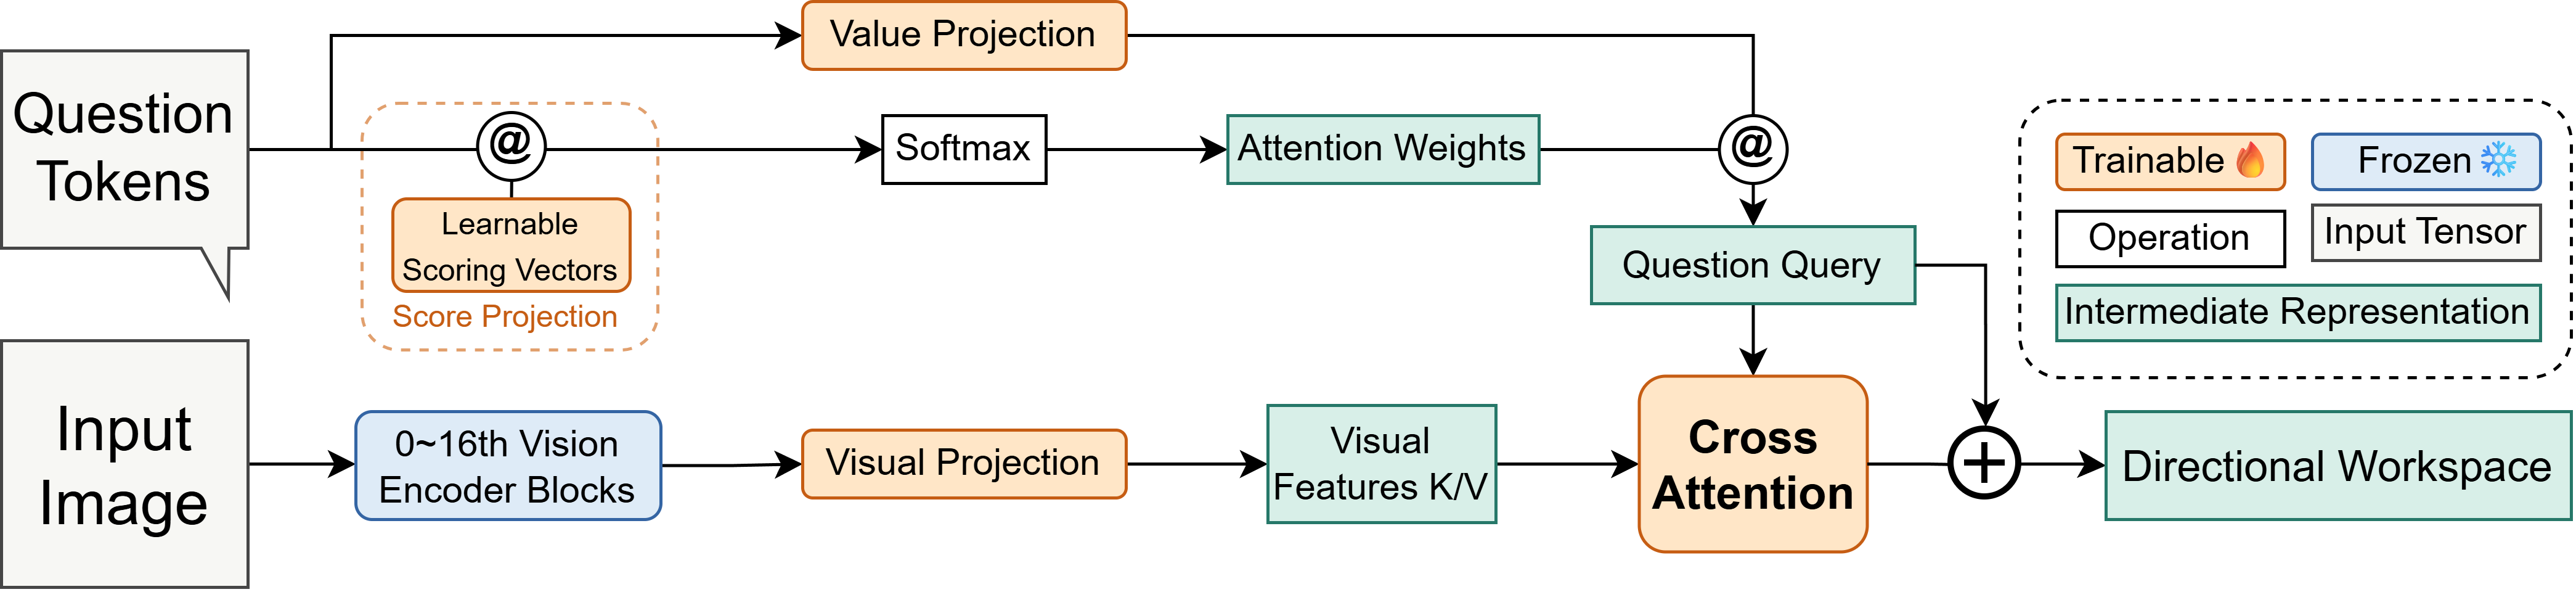
\includegraphics[width=\textwidth]{figures/directional_workspace.png}
    \caption{Directional Workspace的构造。问题Token嵌入经可训练评分向量和Value Projection形成Query；第17层之前的视觉Token投影为K/V。Cross-Attention读取与问题相关的视觉证据，并通过残差连接得到聚合表示。视觉Block采用从0开始的编号，K/V取自索引0至16的Block输出。}
    \label{fig:directional-workspace}
\end{figure}

视觉K/V取自同一样本在第17个视觉Block入口处的图像Token $H^{v}$。通过可训练投影
$W_k,W_v\in\mathbb{R}^{d_v\times D}$得到

\begin{equation}
K=H^{v}W_k,\qquad V=H^{v}W_v.
\end{equation}

以问题表示检索图像区域是视觉问答中的常见建模方式\cite{Anderson2017BottomUpAT,Kim2018BilinearAN}。QDPT采用16头Cross-Attention\cite{Vaswani2017AttentionIA}，以问题表示为Query、图像表示为K/V：

\begin{align}
O &= \operatorname{MHA}(Q,K,V),\\
Z &= Q+O,
\end{align}

其中$Z\in\mathbb{R}^{m\times D}$即Directional Workspace。宽度$D$控制问题投影、视觉投影和跨模态注意力的容量。默认设置为$D=768$。

“Directional”指两种模态在注意力中的固定角色：问题Token形成Query，图像Token只作为K/V。输出$Z$用于生成语言Prompt，不参与视觉编码器后续各层的计算。

\begin{figure}[t]
    \centering
    \begingroup
    \setlength{\unitlength}{\textwidth}
    \begin{picture}(1,0.31187)
        \put(0,0){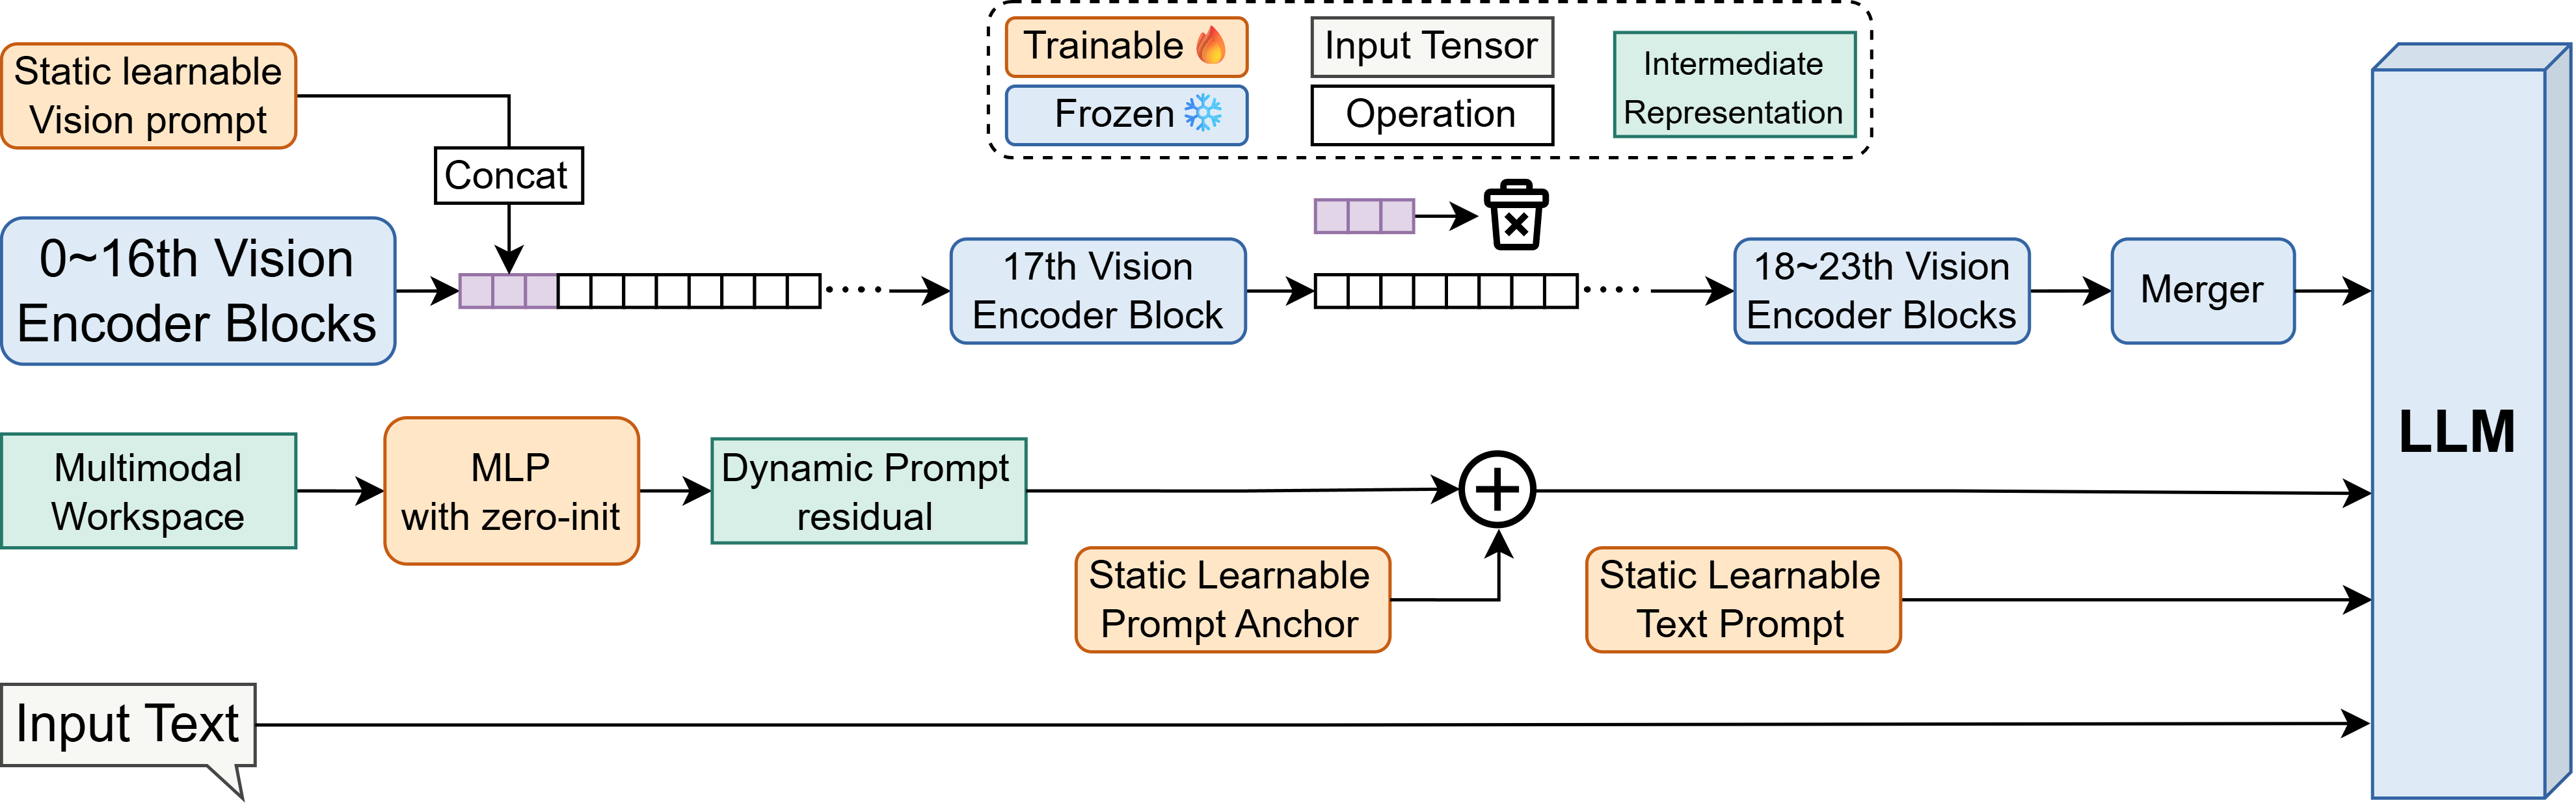
\includegraphics[width=\textwidth]{figures/qdpt_overview.png}}
        \put(0.002,0.099){\color[RGB]{218,239,233}\rule{0.111\textwidth}{0.042\textwidth}}
        \put(0.0575,0.120){\makebox(0,0){\sffamily\resizebox{0.096\textwidth}{!}{\shortstack{Directional\\Workspace}}}}
    \end{picture}
    \endgroup
    \caption{视觉主路径与动态Prompt输出路径。本图承接图\ref{fig:directional-workspace}生成的Workspace。静态视觉Prompt在第17个视觉Block中提供领域校准，并在该层之后移除；问题条件的Directional Workspace只读取视觉证据，经语言侧映射生成动态Prompt。各路输入在LLM入口的排列见图\ref{fig:causal-placement}。视觉Block采用从0开始的编号，第17个Block指索引17。}
    \label{fig:qdpt-overview}
\end{figure}

图\ref{fig:qdpt-overview}承接图\ref{fig:directional-workspace}的聚合结果，展示动态Prompt的生成及其与视觉主路径的衔接。

Directional Workspace通过映射函数
$g_{\theta}:\mathbb{R}^{D}\rightarrow\mathbb{R}^{d_l}$
逐槽转换为语言侧残差：

\begin{equation}
\begin{aligned}
\Delta P^{d}&=g_{\theta}(Z),\\
g_{\theta}(Z)&=\operatorname{GELU}\!\left(\operatorname{LN}(Z)W_1+b_1\right)W_2+b_2.
\end{aligned}
\end{equation}

其中$W_1\in\mathbb{R}^{768\times768}$、$W_2\in\mathbb{R}^{768\times2560}$，映射逐槽执行，两个线性层均含偏置，GELU使用tanh近似。参考零初始化适配器的做法\cite{Zhang2023LLaMAAdapterEF}，输出层的权重与偏置在训练开始时置零，因此初始动态残差为零。模型另维护10个静态可训练Anchor
$A^{t}\in\mathbb{R}^{m\times d_l}$，最终动态Prompt为

\begin{equation}
P^{d}=A^{t}+\Delta P^{d}.
\end{equation}

训练开始时$P^{d}=A^{t}$，随后输出映射逐步学习样本相关的残差。

推理时，动态分支执行问题池化、视觉Cross-Attention和Prompt映射，不针对测试样本进行反向传播。

\subsection{因果输入排列与参数规模}

自回归LLM中的Token顺序会改变各类Prompt能够影响的后续表示。QDPT采用图\ref{fig:causal-placement}所示的输入顺序：静态领域Prompt位于视觉Token之前，问题条件的动态Prompt位于视觉Token之后、问题Token之前。对应的输入序列为

\begin{equation}
E_{\mathrm{LLM}}
= [P^{t};M(I);P^{d};T(X)].
\end{equation}

\begin{figure}[t]
    \centering
    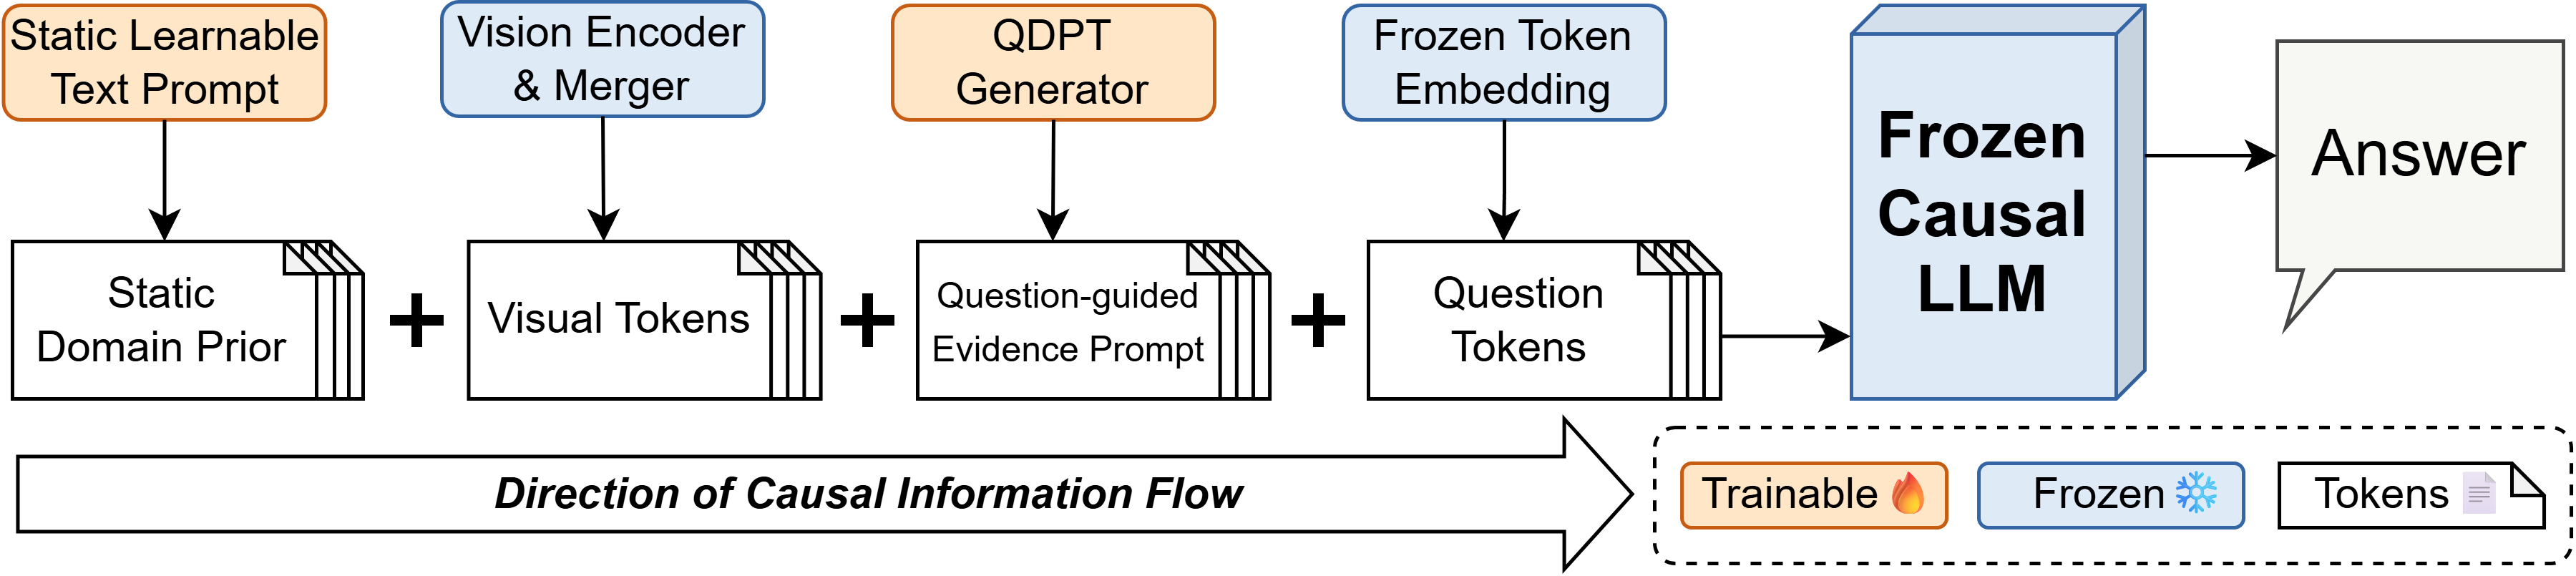
\includegraphics[width=\textwidth]{figures/causal_prompt_placement.png}
    \caption{QDPT在冻结因果LLM中的Prompt放置。静态Prompt位于视觉Token之前，用作领域先验；问题引导的证据Prompt位于视觉Token之后并紧邻问题。箭头表示由因果掩码决定的前向可见方向。}
    \label{fig:causal-placement}
\end{figure}

按照这一顺序，视觉Token能够访问前置的静态Prompt，问题及答案Token能够访问两类Prompt和视觉表示。本文在模型、训练协议和Prompt数量不变的条件下比较其他排列，结果见实验部分。

QDPT共有7,805,184个可训练参数，具体组成见表\ref{tab:trainable-params}。静态语言Prompt、动态Prompt Anchor和静态视觉Prompt合计95,232个参数，占适配器的1.22\%；其余7,709,952个参数用于问题池化、视觉K/V投影、16头Cross-Attention和动态Prompt输出头。

\begin{table}[t]
    \centering
    \caption{QDPT的可训练参数组成。}
    \label{tab:trainable-params}
    \begin{tabular}{lrr}
        \toprule
        模块 & 配置 & 参数量 \\
        \midrule
        静态语言Prompt $P^{t}$ & $20\times2560$ & 51,200 \\
        动态Prompt Anchor $A^{t}$ & $10\times2560$ & 25,600 \\
        静态视觉Prompt $P^{v}$ & $18\times1024$ & 18,432 \\
        问题池化、跨模态检索与输出头 & $D=768$ & 7,709,952 \\
        \midrule
        合计 &  & 7,805,184 \\
        \bottomrule
    \end{tabular}
\end{table}

动态生成器的参数量主要由适配宽度和输出映射决定。输出头压缩的容量对照见附录\ref{sec:output-head-appendix}。训练时，冻结层仍参与前向计算及适配器所需的梯度回传，计算成本还取决于适配参数在骨干中的位置。
